%! TeX root = ../../main-en.tex
% 译自: backmatter/zh/appendix_c.tex @ 9048155:backmatter/zh/appendix_c.tex
\chapter{Writing Bad Code Is Harder Than Writing Good Code}
\label{app:evil-code}

Writing good code is hard: it has to be correct, it has to be clear, and other people have to understand it at a glance. But did you know that writing ``bad'' code on purpose is even harder?

There are two kinds of ``bad'' here. One is \emph{unreadable}: the code runs and gives the right answer, but nobody can tell what it is doing. The other is \emph{underhanded}: the code looks clean and proper, nobody who checks it can find anything wrong, and yet it is quietly up to no good. There are two contests in the world devoted to exactly these two kinds of ``bad''.

The examples for this appendix are in the \texttt{code/en/appc/} directory; the original contest entries that it uses are in \texttt{code/appc/}.

\section{The International Obfuscated C Code Contest}

\subsection{How It Began: Two Pieces of Awful Code}

On 23 March 1984, two programmers at National Semiconductor, Landon Curt Noll and Larry Bassel, were each struggling with a piece of awful code. Bassel was fixing a bug in the Bourne shell (the Unix command interpreter), whose author loved the ALGOL language and had used a pile of macros to ``disguise'' his C code as ALGOL. Noll was fixing a buggy \texttt{finger} program from BSD. The two of them happened to step out into the hallway for a break at the same time, compared notes, and came to the same conclusion: ``the author really had to try to make it this bad!''

So they thought: why not hold a contest to see who can write the worst C program \emph{on purpose}? That is how the \emph{International Obfuscated C Code Contest} (IOCCC) was born.\lazynote{Obfuscate}{To make something deliberately unclear. Obfuscated code is code written on purpose so that nobody can understand it.} The first contest had essentially one rule: write the most obscure complete C program you can, in no more than 512 bytes. It was announced only on Usenet newsgroups in the United States, but when entries started arriving from abroad, the word ``International'' was added to the name.

The contest is still going today; the most recent one was held in 2025. Its website lists the goals of the contest, including ``To show the importance of programming style, in an ironic way'' and ``To emphasize the value of perspicuous code by use of negative examples''. And another one: ``To provide a safe forum for poor C code. :-)''

\subsection{Hello, world from the First Contest}

Here is one of the winning entries from the first contest, in 1984. It is only two lines long. Can you guess what it prints?

\codefile{code/appc/anonymous.c}{A winning entry from the 1984 IOCCC (anonymous author)}{lst:anonymous}

The answer is:
\inputminted[linenos=false]{text}{code/en/appc/out/anonymous.txt}

This program is full of traps:
\begin{itemize}
  \item It defines its own function called \texttt{read}, and inside it calls \texttt{write}---``reading'' is ``writing''.
  \item \texttt{'-'-'-'} is a character minus itself, which is 0; \texttt{'/'/'/'} is a character divided by itself, which is 1. The digits 0 and 1 never appear anywhere in the program, yet 0 and 1 are used all over the place.
  \item \texttt{i["]<i;++i)\{--i;\}"]} looks like a piece of code, but it is really a string. Section~\ref{sec:heap-pointer} explained that \texttt{a[i]} and \texttt{*(a + i)} are the same thing, so \texttt{i["..."]} and \texttt{"..."[i]} are the same thing too.
  \item The string \texttt{"hello, world!"} is split over two lines with a backslash, and the first line ends with \texttt{hell}.
\end{itemize}

The award this entry won was called ``Dishonorable Mention''. The judges wrote: ``The author was too embarrassed that they could write such trash, so I promised to protect their identity.'' To this day, the author's name is still a secret.

It is written in the old-fashioned C of 1984, so today's compilers need to be told to compile it like this (\texttt{-w} switches off a whole pile of warnings):
\begin{minted}[linenos=false]{text}
gcc -m32 -std=gnu89 -w anonymous.c -o anonymous
\end{minted}

\subsection{Obfuscating Something Ourselves}

Let's have a go ourselves. Here is a program that prints a triangle, written the proper way:

\codefile{code/en/appc/triangle_good.c}{Printing a triangle: the well-behaved version}{lst:tri-good}

And here is one that does exactly the same thing and prints exactly the same output:

\codefile{code/en/appc/triangle_evil.c}{Printing a triangle: the ``obfuscated'' version}{lst:tri-evil}

It uses a few little tricks: \texttt{putchar} is hidden inside a macro called \texttt{\_}; the variables are called \texttt{\_\_} and \texttt{\_\_\_} (two and three underscores, both perfectly legal names in C); \texttt{42} and \texttt{10} stand in for \texttt{'*'} and \texttt{'\textbackslash n'} (their character codes happen to be 42 and 10); and the newline is tucked into the third part of a \texttt{for} loop. And this is only beginner level---real IOCCC entries are a hundred times harder to read.

\subsection{Some Famous Entries and Stories}

\paragraph{A program with no bytes at all.}
There is a kind of program called a \emph{quine}:\lazynote{Quine}{A program that prints its own source code when it runs.} when you run it, it prints its own source code, exactly. Almost every year someone sent in ``the world's shortest self-reproducing program'', and the judges could tell at a glance that it was not short enough. Then, in 1994, Szymon Rusinkiewicz sent in a file called \texttt{smr.c}. It was empty: 0 bytes. An empty program prints nothing when it runs, and what it prints is exactly its own source code: 0 bytes. The judges gave it the award for ``Worst abuse of the rules'', and then changed the rules: ``In the future, the contest rules will specify a minimum size that is one character larger than this entry.''

\paragraph{All sorts of strange awards.}
The awards the IOCCC hands out every year have wonderful names: ``Worst abuse of the C preprocessor'', ``Most unpredictable behavior'', ``Best one-liner''\ldots{} Among the winners are programs that play chess, programs that fly a flight simulator, programs that compute $\pi$---and one whose source code, laid out with underscores and minus signs, is simply a big circle, and what it computes is $\pi$.

\begin{figure}[htbp]
  \centering
  \begin{tikzpicture}[line width=0.8pt]
    % A tangled mess of code
    \node[draw, fill=yellow!10, font=\ttfamily\scriptsize, align=left, inner sep=4pt] (code) at (0,0)
      {\#define \_(x) putchar(x)\\int main(void)\{int \_\_=0,\_\_\_;\\for(;\_\_++<5;\_(10))\\for(\_\_\_=\_\_;\_\_\_--;\_(42));\}};
    % A little person reading the code
    \draw (3.4,0.5) circle (0.22);
    \draw (3.4,0.28) -- (3.4,-0.5);
    \draw (3.4,-0.5) -- (3.2,-1.1) (3.4,-0.5) -- (3.6,-1.1);
    \draw (3.4,0.1) -- (3.1,0.4) -- (3.2,0.65);
    \draw (3.4,0.1) -- (3.7,-0.15);
    \node[font=\Large\bfseries, text=lazyred] at (3.75,0.95) {?};
    \node[draw, rounded corners, fill=white, font=\small] at (4.9,1.7) {This\ldots{} is C?};
    \node[font=\scriptsize, gray] at (0,-1.1) {(It really does compile. And run.)};
  \end{tikzpicture}
  \caption{What reading an IOCCC entry feels like}
  \label{fig:ioccc}
\end{figure}

\section{The Underhanded C Contest}

\subsection{Scarier Than ``Unreadable''}

With IOCCC code, anyone can see at a glance that something is wrong: who would write a serious program like that? What is really frightening is code that \emph{looks perfectly fine}.

That is what the \emph{Underhanded C Contest} is all about.\lazynote{Underhanded}{Done in secret and dishonestly; sneaky.} It is run by Scott Craver of Binghamton University in the United States, and it describes itself like this: ``In many ways this is the exact opposite of the Obfuscated C Code Contest.'' The code you submit must be ``as readable, clear, and seemingly trustworthy as possible'', and yet it must secretly do something bad. Better still, even if someone spots it, it should be easy to pass off as an innocent bug: ``Bugs are worth more points if, once discovered, they are plausibly deniable as an innocent programming error.'' The point of the contest is to show people that important programs need careful code review.

Every contest has a theme, for example: quietly leaving out a few votes when counting an election; quietly skimming a little off the top when processing financial transactions; secretly leaking information to an eavesdropper\ldots{}

\subsection{Two Famous Winners}

\paragraph{2008: Blacked out, but not quite.}
The task was to write a program that ``redacts'' an image: it blacks out a given area of the picture (a face in a photo, say, or the secret part of a document), but in a way that secretly lets the blacked-out content be recovered. The contest received more than a hundred entries, and the winner was John Meacham. Here is his entry. Even with comments, it is only fifty-odd lines long (when the author published it on his blog, he left out the \texttt{\#include} lines at the top; this book has added the first 6 lines):

\codefile{code/en/appc/redact.c}{2008 winner: John Meacham's redaction program}{lst:redact}

It works on images in a text format (the P3 variant of PPM): the file starts with the width, the height and the maximum brightness, and after that each pixel is written as three decimal numbers for red, green and blue, where 0 is darkest and 255 is brightest. The program first copies the header unchanged (lines 34 and 35), then reads the file one line at a time (line 43), and looks at each line one character at a time (line 44):
\begin{itemize}
  \item When it meets a digit (line 45) that starts a new number, it adds one to the position \texttt{x}, moving on to the next row when the current row is full (lines 46--51). The variable \texttt{ws} remembers whether we are ``in the middle of a number right now''.
  \item If that position is inside the rectangle to be blacked out (line 52), it prints the character \texttt{'0'} (line 53); otherwise it prints the digit unchanged.
  \item Characters that are not digits, such as spaces and newlines, are printed unchanged (lines 57 and 58).
\end{itemize}

The flaw is in line 53: it replaces \emph{every digit character} with \texttt{'0'}, instead of replacing \emph{every number} with \texttt{0}. Let's try it on a small image, 4 columns by 3 rows, and black out the second row:
\begin{minted}[linenos=false]{text}
$ ./redact secret.ppm 0 0 4 2
\end{minted}
\inputminted[linenos=false]{text}{code/en/appc/out/redacted.ppm}

Where there used to be \texttt{7 7 7} (very dark), there is now \texttt{0 0 0}; where there used to be \texttt{60 60 60}, there is now \texttt{00 00 00}; and where there used to be \texttt{255} (brightest), there is now \texttt{000}. In an image viewer they all look black, with no difference at all. But open the file and count the zeros, and you know whether each number used to have one, two or three digits---in other words, roughly how bright it used to be. Redaction is most often used on documents with black text on a white background, where every number is either 0 or 255, so the blacked-out text can be recovered \emph{perfectly}.

(Sharp-eyed readers will notice that the last number, \texttt{255}, was not blacked out. That is because the row check in line 48 puts \texttt{x} and \texttt{y} one step out of step at the end of each row. It is a small glitch in the original entry, and has nothing to do with the sneaky part.)

Why process the image one character at a time, instead of the more natural \texttt{scanf("\%d \%d \%d", ...)}, reading one number at a time? Meacham said on his blog that this was the part he was proudest of: if anyone challenged him, he would answer that it was to avoid the notorious buffer overflow pitfalls of \texttt{gets} and \texttt{fgets} (the comment ``fixed buffer size to avoid overflow'' in line 40 is there to prepare the ground). Something that looks like it was written for \emph{safety} is exactly where the hole is. The judges praised it as a perfect illustration of the spirit of the contest: ``make the code extremely simple, innocent, obvious, and wrong.''

\paragraph{2015: Inspecting nuclear warheads.}
This contest was run together with an organization that works against the spread of nuclear weapons, and the task was a serious one. Two countries have signed a nuclear disarmament treaty. A program compares the gamma-ray spectrum of a warhead with a reference spectrum and prints only ``yes'' or ``no'': is this a real nuclear warhead? Entrants had to make the program also say ``yes'' to a fake warhead under some condition that can be set up on purpose---so that a country could hand over fake warheads and secretly keep the real ones.

The winner was Linus Åkesson. His entry is just three files, 72 lines in all. First, the header file:

\codefile{code/appc/match.h}{2015 winner: match.h}{lst:match-h}

Next, the main logic. \texttt{match} makes two checks. First it compares the totals of the two spectra (line 40): if the fake warhead has too little nuclear material, the answer is ``no'' straight away. Then it smooths each spectrum, takes the differences, and smooths again (\texttt{preprocess}, lines 30--35), and finally compares whether their ``shapes'' are alike (line 43):

\codefile{code/appc/match.c}{2015 winner: match.c}{lst:match-c}

The last file works out how similar the two spectra are: it treats them as two vectors, divides each by its own length (\texttt{normalize}), and takes their dot product (\texttt{dot\_product}). The more alike the two vectors are, the closer the result is to 1:

\codefile{code/appc/spectral_contrast.c}{2015 winner: spectral\_contrast.c}{lst:spectral}

Three files, and every line looks beyond reproach. The secret is hidden in the \texttt{\#include} lines at the top of two of the files:
\begin{itemize}
  \item \texttt{match.c} includes \texttt{match.h}, which says \texttt{typedef double float\_t;}. So as far as \texttt{match.c} is concerned, \texttt{float\_t} is an 8-byte \texttt{double}.
  \item \texttt{spectral\_contrast.c} includes only \texttt{<math.h>}. The standard library's \texttt{math.h} \emph{already} defines a \texttt{float\_t} of its own, and on x86-64 it is a 4-byte \texttt{float}.
\end{itemize}
The two files are compiled separately. The compiler looks at each one on its own and never learns that the other file's \texttt{float\_t} is different, so it says nothing. But \texttt{match} hands an array of 8-byte numbers to \texttt{spectral\_contrast}, which reads it as 4-byte numbers (Section~\ref{sec:heap-pointer} explained that how far a pointer moves when you add one depends on the type of the elements). As a result:
\begin{itemize}
  \item Only the \emph{first half} of the array is read: \texttt{length} 4-byte numbers are exactly the first \texttt{length/2} 8-byte numbers. The second half of the spectrum takes no part in the comparison at all.
  \item Each 8-byte \texttt{double} is read as two 4-byte pieces, giving ``squashed'' values that have almost nothing to do with the original sizes. Big peaks and small peaks are squashed to roughly the same height, so you can hardly tell any more whether the shapes match.
\end{itemize}

And that gives us a way to cheat: put just a tiny amount of real nuclear material in the fake warhead, so that the ``shape'' of the first half of the spectrum matches; then add a very strong signal in the second half, so that the check on the total (line 40---this step is done in \texttt{match.c}, which is not fooled) passes too. This book includes a small program to try it out (\texttt{code/en/appc/inspect.c}, not part of the original entry): the fake warhead has only 3\% of the nuclear material of the reference spectrum, plus a strong, unrelated peak in the second half. Here is what it prints:
\inputminted[linenos=false]{text}{code/en/appc/out/inspect.txt}

The fake warhead passes! If the two files agree about \texttt{float\_t}---for example, if you replace the \texttt{\#include <math.h>} at the top of \texttt{spectral\_contrast.c} with \texttt{\#include "match.h"} (and declare \texttt{sqrt} yourself)---the fake warhead is caught and gets a \texttt{FAIL}. Interestingly, if both headers are included \emph{at the same time}, the compiler does complain: \texttt{float\_t} is defined twice, with two different types. The author carefully made sure that each file includes only one of them.

The judges said that ``beyond that type confusion, the code does nothing unusual or suspicious or quirky or different: it is a bog-standard implementation of preprocessing followed by normalized correlation'', so it ``looks incredibly innocent''. Even if the trick were discovered, it would be easy to blame on an accident: who would have guessed that \texttt{math.h} has a \texttt{float\_t} too? The author's write-up of the entry (with all the code) is at \url{https://www.underhanded-c.org/one.pdf}.

\subsection{Let's Be Underhanded Too}

The function below checks whether a user is an administrator. Look carefully: what is wrong with it?

\codefile{code/en/appc/admin.c}{Checking for an administrator: looks perfectly normal}{lst:admin}

\inputminted[linenos=false]{text}{code/en/appc/out/admin.txt}

Everybody is an administrator! The trouble is in lines 11--13: there are no braces after the \texttt{if}, so it controls only the \emph{one} statement right after it, the \texttt{printf}. The \texttt{admin = 1;} on the next line is indented just like the \texttt{printf}, but the \texttt{if} has no say over it at all; it runs every time. The indentation fools the eye, but the compiler does not look at indentation.

Now look at a program that counts votes:

\codefile{code/en/appc/vote.c}{Counting votes: cat versus dog}{lst:vote}

\inputminted[linenos=false]{text}{code/en/appc/out/vote.txt}

Out of 8 votes, the dog clearly got 5, yet every single vote went to the cat. The culprit is \texttt{ballots[i] = 1} in line 12: one equals sign is missing, so ``check whether it equals 1'' has become ``store 1 in it'' (Section~\ref{sec:logic} warned you about this). Not only does it count every vote ``for the cat'', it also changes the ballots themselves, so you cannot even count them again afterwards.

\subsection{This Is Not Just a Game}

Both of these tricks have happened in the real world.

\paragraph{Apple's ``goto fail''.}
In 2014, Apple released an urgent security update. The problem was in the code that checked HTTPS certificates on iOS and macOS, where a line \texttt{goto fail;} had been written twice:
\begin{minted}[linenos=false]{c}
if ((err = SSLHashSHA1.update(&hashCtx, &signedParams)) != 0)
    goto fail;
    goto fail;
\end{minted}
The second \texttt{goto fail;} is just like \texttt{admin = 1;} in \texttt{admin.c}: the indentation makes it look as if it belongs to the \texttt{if}, but it actually runs every time. So the most important step after it, checking the signature, was skipped entirely---and at that point the variable that records errors was still 0, meaning ``all is well''. As a result, an attacker could pretend to be any HTTPS website at all. Nobody knows whether this was a careless copy-and-paste mistake or done on purpose.

\paragraph{The 2003 Linux backdoor.}
In November 2003, someone secretly modified a copy of the Linux kernel source code, adding two lines to the \texttt{wait4} system call:
\begin{minted}[linenos=false]{c}
if ((options == (__WCLONE|__WALL)) && (current->uid = 0))
        retval = -EINVAL;
\end{minted}
It looks as if it checks ``is the current user the superuser?'' (\mbox{\texttt{uid == 0}}), but in fact it \emph{makes} the current user \emph{into} the superuser (\mbox{\texttt{uid = 0}}). Any ordinary program could quietly gain the highest privileges just by calling \texttt{wait4} with two special arguments. The author even added an extra pair of parentheses on purpose, because that stops the compiler from giving a warning. Luckily, the change had no matching record of approval, and it was soon discovered. To this day, nobody knows who did it.

\begin{figure}[htbp]
  \centering
  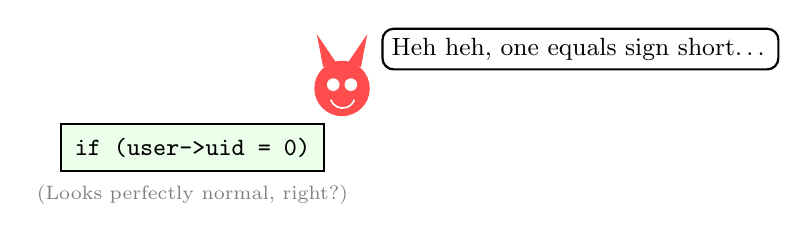
\begin{tikzpicture}[line width=0.8pt]
    % A neat and tidy line of code, with a little devil hiding behind it
    \node[draw, fill=green!8, font=\ttfamily\small, inner sep=5pt] (c) at (0,0)
      {if (user->uid = 0)};
    % The little devil: peeking out from the top right corner of the code box
    \begin{scope}[shift={(1.9,0.75)}, scale=1.6]
      \fill[red!70] (0,0) circle (0.22);
      \fill[red!70] (-0.15,0.17) -- (-0.2,0.43) -- (-0.05,0.21) -- cycle;
      \fill[red!70] (0.15,0.17) -- (0.2,0.43) -- (0.05,0.21) -- cycle;
      \fill[white] (-0.07,0.03) circle (0.05) (0.07,0.03) circle (0.05);
      \draw[white, line width=0.6pt] (-0.09,-0.09) arc[start angle=200, end angle=340, radius=0.1];
    \end{scope}
    \node[draw, rounded corners, fill=white, font=\small, anchor=west] at (2.4,1.25) {Heh heh, one equals sign short\ldots{}};
    \node[font=\scriptsize, gray] at (0,-0.6) {(Looks perfectly normal, right?)};
  \end{tikzpicture}
  \caption{Underhanded code}
  \label{fig:underhanded}
\end{figure}

\section{How to Deal with Bad Code}

The two little tricks in this appendix have one thing in common: the compiler can actually spot them. Our Makefile deliberately leaves out \texttt{-Wall}. Add it, and \texttt{gcc} says this:
\inputminted[linenos=false, fontsize=\scriptsize]{text}{code/en/appc/out/wall.txt}

The first warning says that this \texttt{if} does not guard the indented lines below it: the indentation is lying (``misleading indentation''). The second is the same warning we met in Section~\ref{sec:logic}.

So the way to deal with bad code is simply the set of good habits this book has been talking about all along:
\begin{itemize}
  \item turn on warnings when you compile (\texttt{-Wall -Wextra}), and read every one of them carefully;
  \item always put braces after an \texttt{if}, even when there is only one statement;
  \item write tests, so that the program checks its own results automatically---that is what \texttt{make test} does in every chapter of this book;
  \item ask other people to read your code. The Underhanded C Contest teaches us that a problem one person cannot see may well be spotted when two or three people look carefully.
\end{itemize}

Writing good code is hard; writing bad code is even harder. Luckily, seeing through bad code is a skill you can learn.
